\subsection*{La Culture de la Collaboration et de la Flexibilité}
\subsubsection{Méthode de Travail}
Amiral Technologies opère selon une approche agile, organisée en cycles de travail appelés sprints, d'une durée de 4 à 6 semaines.

Chaque sprint est composé de plusieurs épics (grandes fonctionnalités) rassemblant des tâches liées à un même thème.
À la clôture d'un sprint, une réunion de rétrospective est organisée pour obtenir des retours sur la période écoulée et évaluer les progrès des projets.
De plus, une activité ludique ou un jeu de société est souvent intégré à la réunion, favorisant ainsi la détente et le renforcement de l'esprit d'équipe au sein du département de développement.

Des réunions trihebdomadaires sont également programmées pour créer des opportunités d'échanger sur les avancées immédiates et de discuter des éventuels obstacles rencontrés par les développeurs.
Ces réunions régulières offrent un contexte propice à la résolution collaborative des problèmes et à la génération d'idées.


\subsubsection{Environnement de Travail}
\begin{figure}[ht!]
    \begin{minipage}[c]{0.475\textwidth}
        Les locaux d'Amiral Technologies sont aménagés en un vaste open space comportant une vingtaine de bureaux, ainsi que deux salles de réunion.
        
        Les heures de travail varient en fonction des préférences individuelles, avec un consensus autour d'une arrivée vers 9h30 et d'un départ entre 17h00 et 18h00.
        
        Deux jours de télétravail sont accordés chaque semaine aux employés qui le souhaitent.
        Pour ma part, j'optais généralement pour le travail au bureau en effectif réduit.
    \end{minipage} %
    \begin{minipage}[c]{0.05\textwidth}
        \hfill
    \end{minipage} %
    \begin{minipage}[c]{0.475\textwidth}
        \centering
        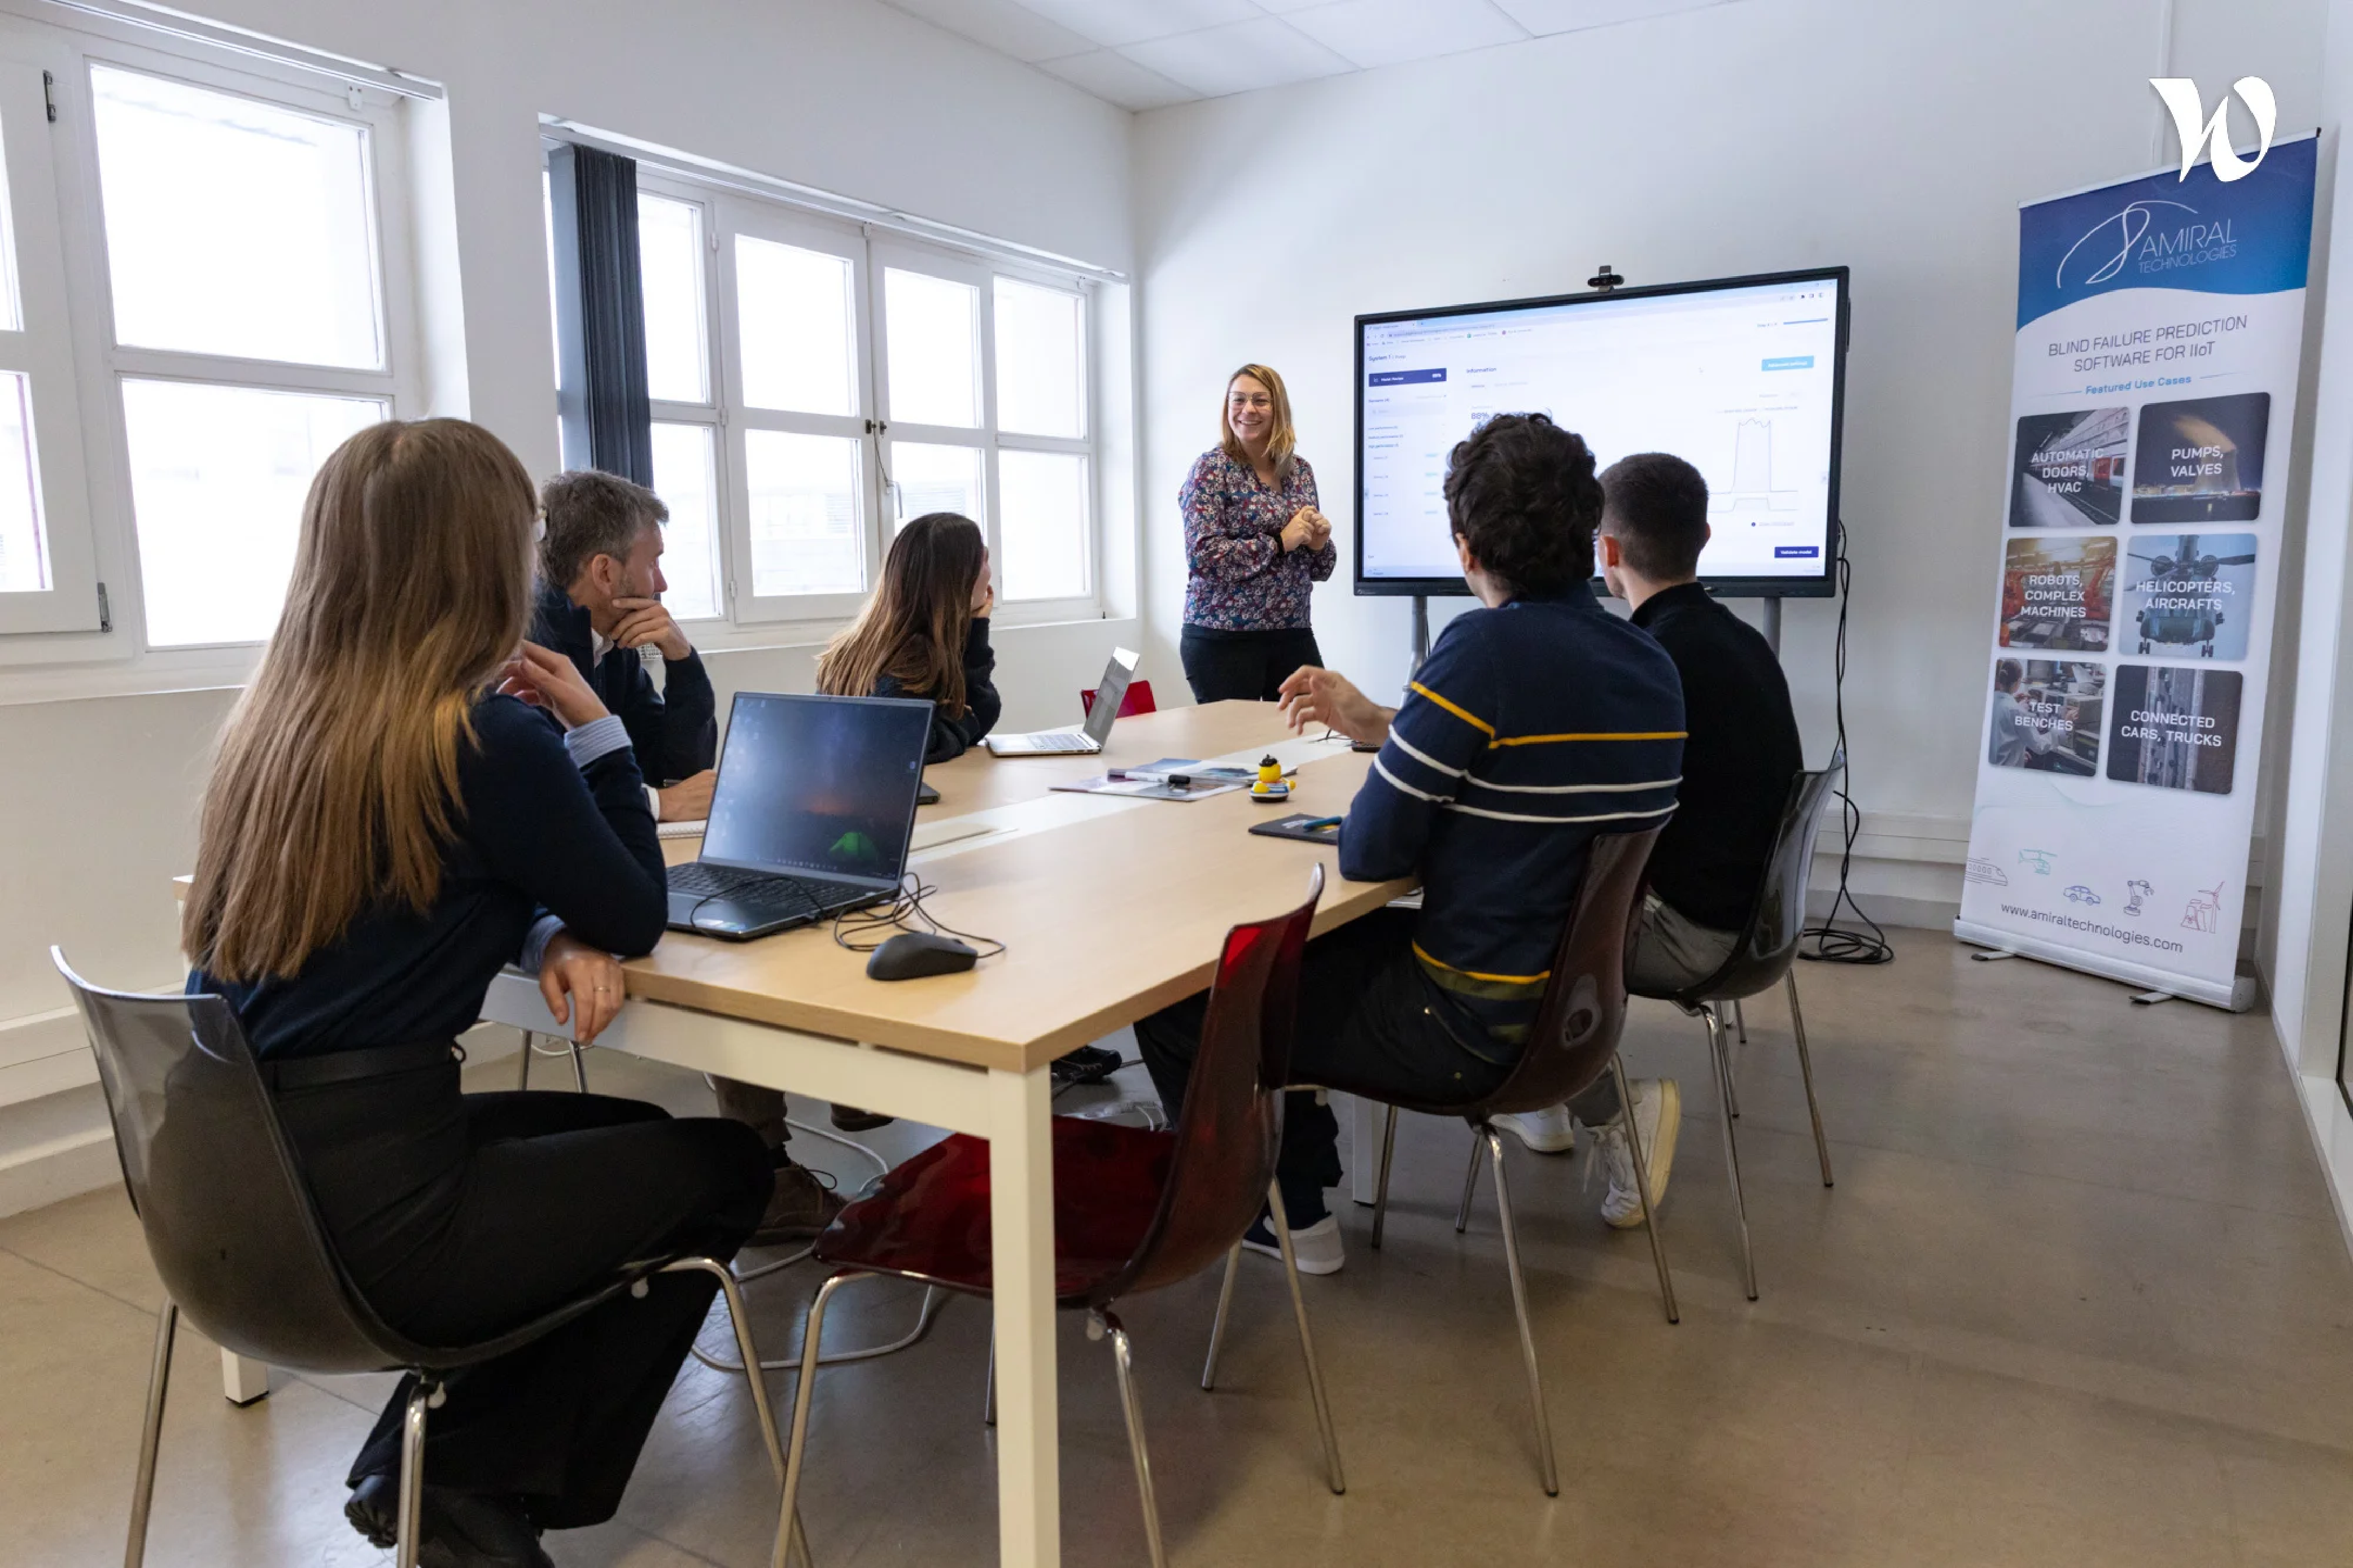
\includegraphics[width=\textwidth]{paper/figures/equipe-prez.pdf}
        \caption{Réunion d'équipe}
    \end{minipage}
\end{figure}